\documentclass{rapport}

%----------------------------------------
% Propriétés du document
%----------------------------------------
\author{Jonathan \textsc{Bregnard},\\Igor \textsc{Ayrton}}
\footauthor{J. \textsc{Bregnard}, I. \textsc{Ayrton}}
\semester{MT MA1}
\cours{Projet de semestre}
\teacher{Prof. M. Bouri}
\date{juin 2015}
\title{China Hardware Innovation Camp - Vesta}
\subtitle{Engineering Report}

%----------------------------------------
% Index et glossaire
%----------------------------------------
%\makeindex
%\makegloss

\begin{document}

% Titre
%----------------------------------------

\maketitle
%\thispagestyle{empty}
%\clearemptydoublepage

%----------------------------------------
% Table des matières
%----------------------------------------


\pagenumbering{roman}
\toc

%\clearemptydoublepage

%----------------------------------------
% Contenu
%----------------------------------------
\setcounter{page}{1}
\pagenumbering{arabic}
\section{Introduction}

This semester project takes part of the CHIC2015 which is a new project initiated at EPFL by Marc Laperrouza. The goal of this new project is for students develop a project from idea to production in a semester. Indeed a trip to Shenzhen in China is programmed following the end of the semester(july). The prototype will be produced by chinese company called Seeedstudio. They mainly do pcb prototyping but they also mill and 3d print parts.

Three groups of 5 people are created after a brainstorming week-end at the beggining of the semester with for each group one HEC (economy) student, one ECAL (industrial design) student and three engineering students from EPFL. For the project presented in this report, two engineers are from microengineering and one is from material science.

The economy student works on the buisness part of the project which contains the buisness model, the market definition and the value proposition. The industrial design student works on the mecanical and software design. The engineering students work on the materials, hardware and software of the project.

After the brainstorming week-end, the rough idea was to connect elderly people to their families with an easy to use electronic device. Many elderly people are excluded from the new technologies and are therefore excluded from modern communications.

In this report, the focus will be put on the engineering part of the project especially. An abstract to the market researches will be introduced. The industrial design and the material parts will also be discussed to have a global aspect of the project.

\section{Problem and Solution}
In this section we will lay out the problematic we wanted to adress during this project. Our chosen solution wil be introduced and described.
\subsection{Problem}
\subsection{Solution}
\subsection{Vesta tab}
The Vesta tab is a tablet oriented towards the elderly. It has a capacitive touch screen, a wifi and bluetooth connection and a unique casing. The main usage at the moment is receiving and displaying pictures and text sent by the younger family via the dedicated website. As soon as a new image or text is received an LED blinks to inform the user of new content. The interface is designed to be very user friendly and easy to use.
\section{Value Proposition and Buisness Model}

\subsection{Value Proposition}

\subsection{Buisness model}

The buisness model is shown in the figure \ref{fig:buisness model}.

\begin{figure}[!htb]
    \centering
    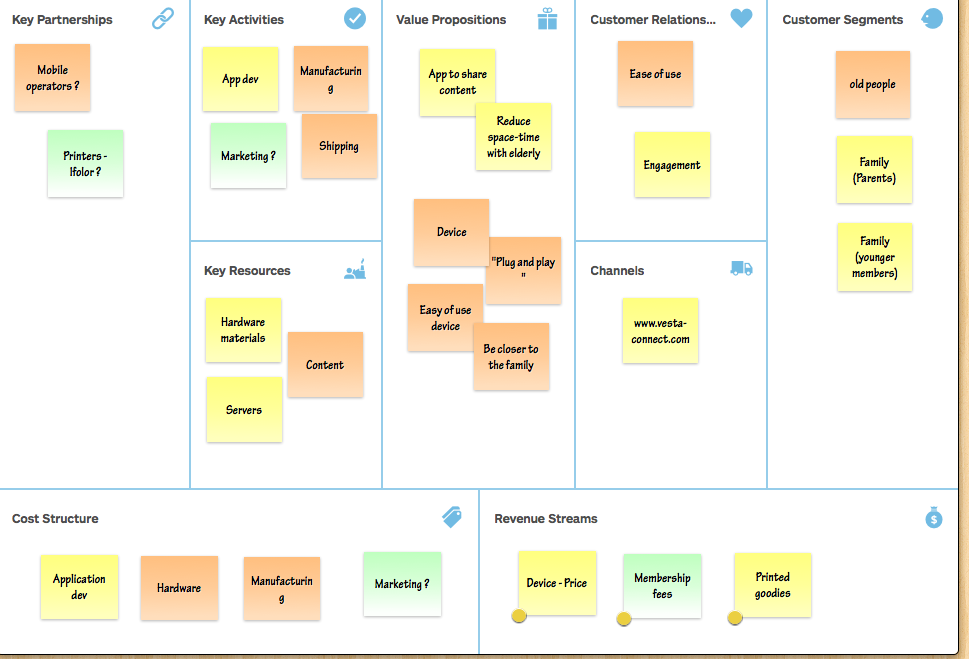
\includegraphics[width=0.9\textwidth,keepaspectratio]{chap/buisnessFig/buisness_model.png}
    \caption{Buisness model}
    \label{fig:buisness model}
\end{figure}

\subsection{User tests}


\section{Industrial design}

In this section, the industrial design will be explained and especially shown with pictures to have an idea of how the product will look. The design part was done by the ECAL student. The indutrial designer presented different solutions, they were then discussed together with the other member of the group. The solutions were also presented to the nurses and some old people to define which one is the more understandable and easy to use.

\subsection{Tablet}


The design of the tablet is shown in the figure \ref{fig:vesta design}.

\begin{figure}[!htb]
    \centering
    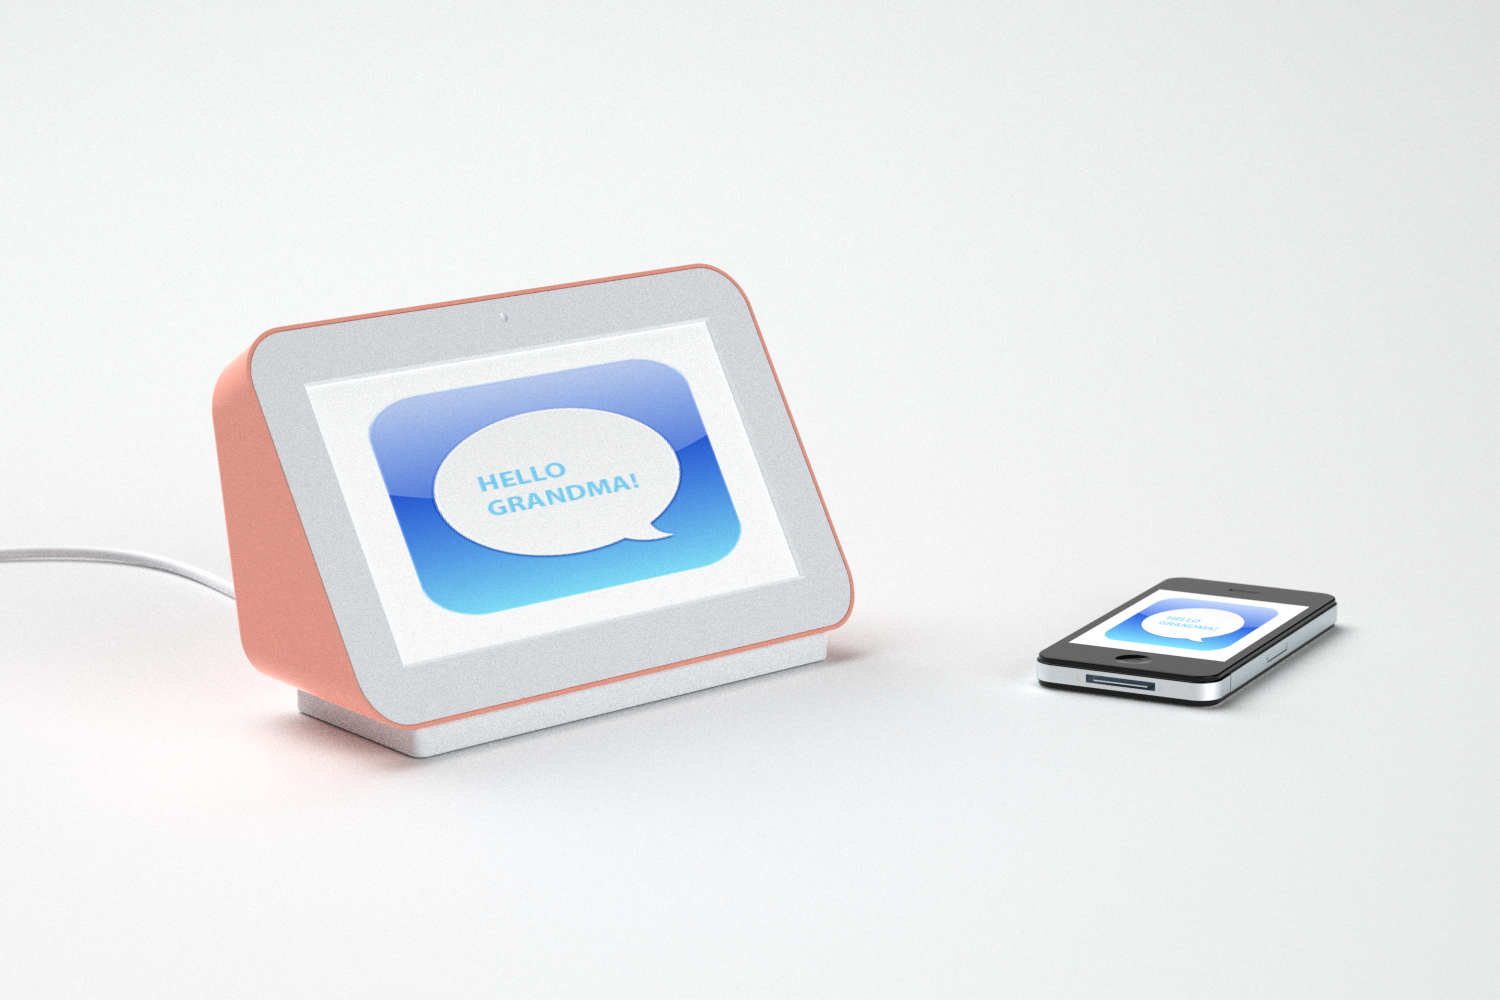
\includegraphics[width=0.9\textwidth,keepaspectratio]{chap/designFig/VestaRender4.png}
    \caption{Vesta tablet design}
    \label{fig:vesta design}
\end{figure}


\subsection{Charging station}

\begin{figure}[!htb]
    \centering
    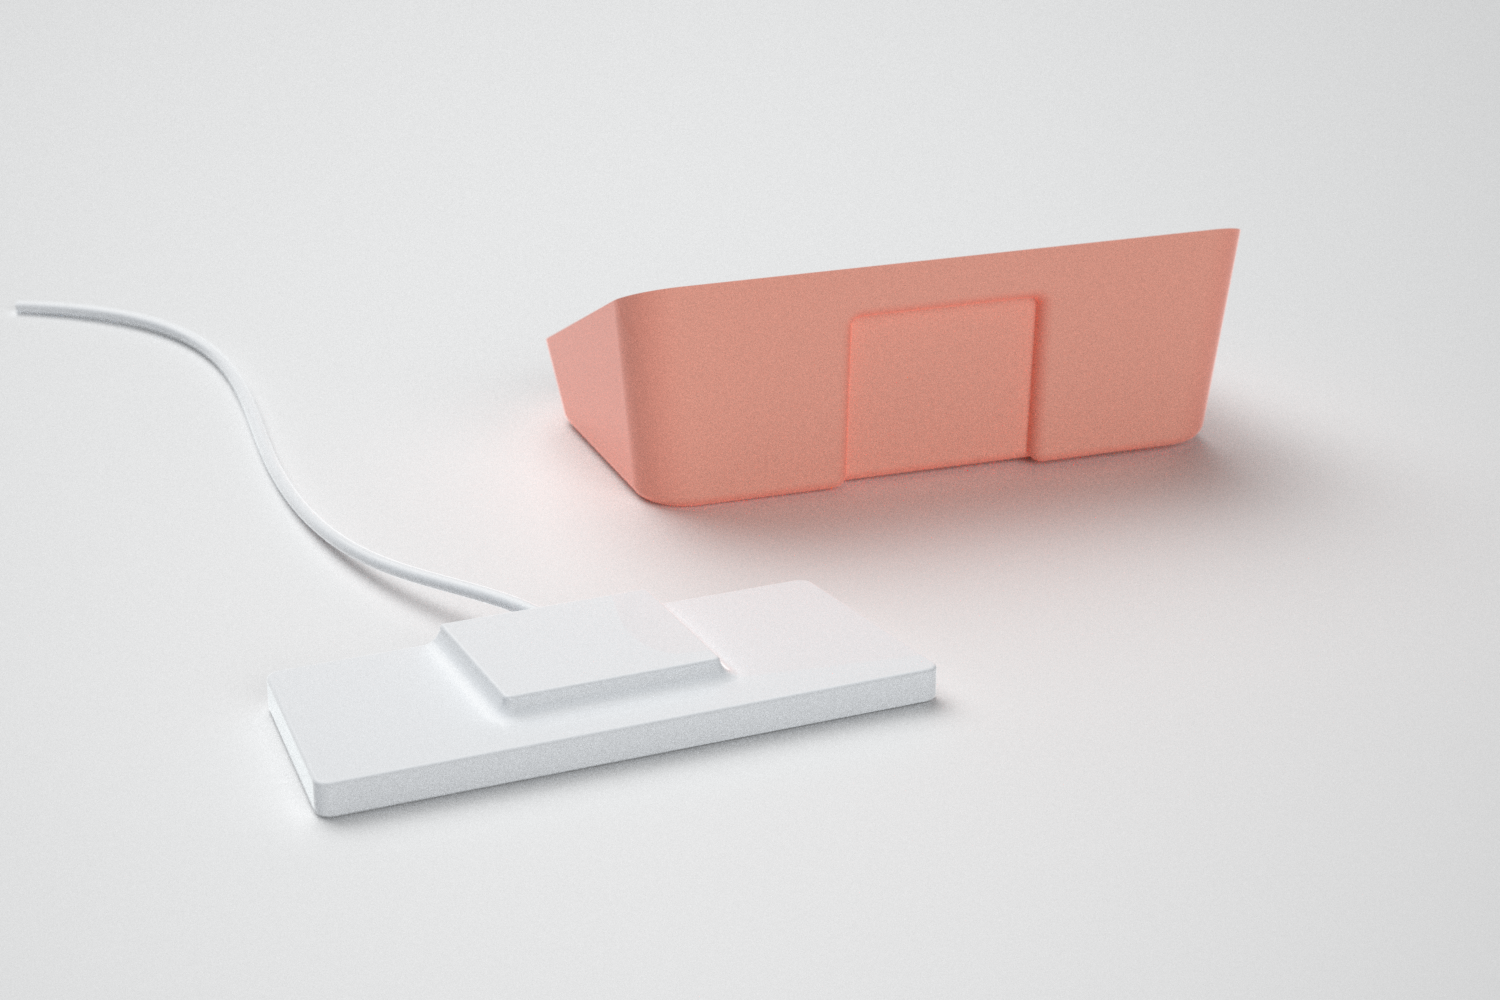
\includegraphics[width=0.9\textwidth,keepaspectratio]{chap/designFig/VisioRender7.png}
    \caption{Charging station}
    \label{fig:charging station}
\end{figure}

\clearpage

\subsection{Software design}

The graphical interface of the software is shown in the figure \ref{fig:soft design}.

\begin{figure}[!htb]
    \centering
    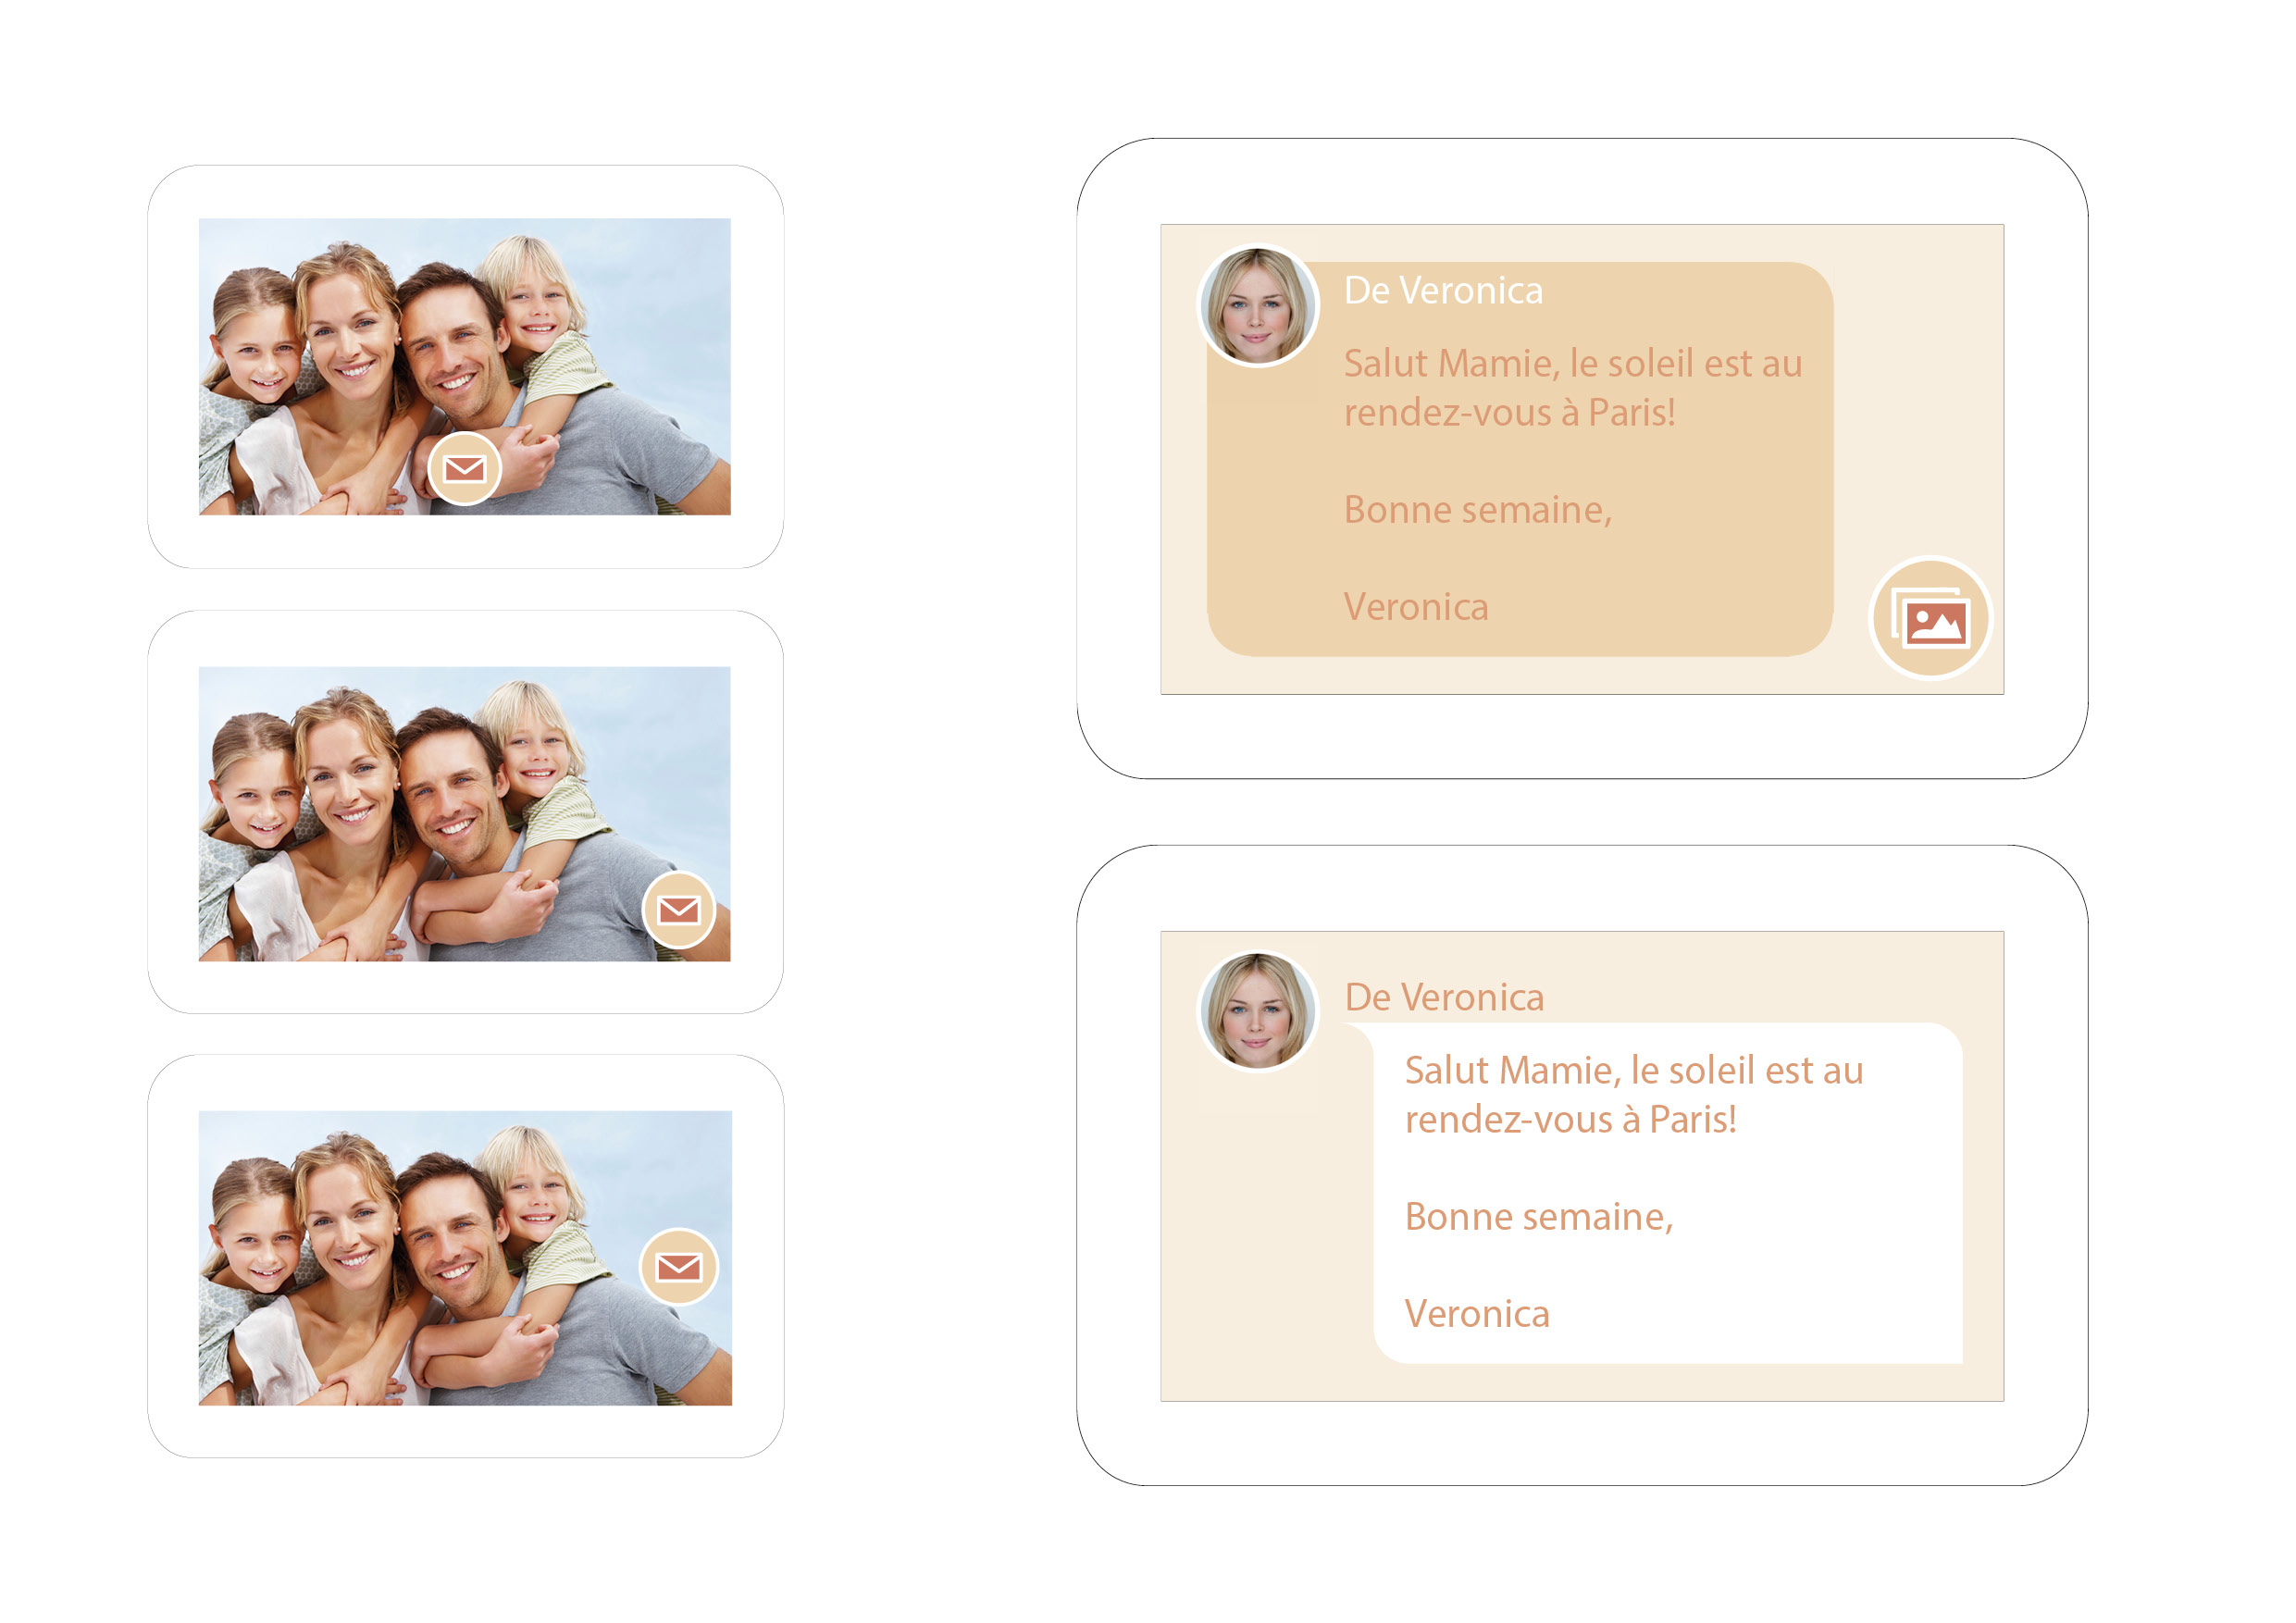
\includegraphics[width=0.9\textwidth,keepaspectratio]{chap/designFig/vesta_design.jpg}
    \caption{Software design}
    \label{fig:soft design}
\end{figure}

\section{Materials}
\section{Hardware}

This section is dedicated to show all the electronic components we chose and how they work together. As described earlier the PCB containing all the components will be manufactured by Seeedstudio. They manufacture PCBs with other hardware components and they sell quite a number of different breakout boards and other developpement parts. A request made by CHIC managing team was to source as many components as possible at Seeedstudio. Of course not all components we needed were available by them so some of the components are from different sources.

We were basically going to build a tablet. It didn't need to have the power of high end tablets of today but it still was quite a challenge. At first we were thinking it would be possible to take an open source ARM chip devellopment board, devellop our application and then take the schematics and rebuild a whole board including the processor, memory, etc.. plus all our peripherals and build the whole device from scratch. But we quickly understood that it was much too complicated to do in a semester. So we decided to take an existing board and build an add-on board hosting our additionnal components.

There are a number of different devellopment/tinkering boards out there. The most famous one might be the raspberry Pi, although quite capable it seemed a little limited for our application (clocked at 700 mhz for the raspberry pi 1). Another problem was that the raspberry pi is not completely open source. Indeed its schematics and gerber files are not available. At the beginning of the project thinking we might build the whole board up from scratch it was necessary for us to work with a totally open source platform which we could build upon.

So we looked into one of the other famous board: the beagle bone black. Which we will further refer to as the BBB. This board clocked at 1 GHz seemed quite capable. There was lots of documentation, a wide community, and especially it is completelly open source hardware and software. This is what we went for.

In fig.\ref{fig:hardware dependencies} we describe the different components of our device and how the connect to each other.

\begin{figure}[!htb]
    \centering
    \includegraphics[width=0.7\textwidth,keepaspectratio]{chap/hardFig/overall_hardware_dependecies}
    \caption{Hardware components dependencies.}
    \label{fig:hardware dependencies}
\end{figure}

\subsection{Beaglebone Black}
The BBB uses an ARM processor from Texas Instruments, the AM335X. It is clocked at 1GHz.
\begin{itemize}
  \item{ AM335x 1GHz ARM® Cortex-A8 }
  \item{512MB DDR3 RAM}
  \item{4GB 8-bit eMMC on-board flash storage}
  \item{Ethernet}
  \item{2x 46 pin headers}
  \item{Open source}
  \item{...}
\end{itemize}



% \begin{table}[!htbp]
%   \begin{center}
%     \begin{tabular}{|l|r|r|}%p{5cm}|}
%       \hline
%         measurement N$^{\circ}$ & CW [mNm] & CCW [mNm]\\ \hline %\hline
%         test two & 2.24e-4 & -6.32e-4 \\ \hline
%         2 & 2.073-4 & -6.39e-4\\ \hline
%         3 & 2.72e-4 & -6.64e-4\\ \hline
%         4 & 2.46e-4 & -6.46e-4\\ \hline
%         5 & 2.72e.4 & -6.64e-4\\ \hline \hline
%         mean & 2.44e-4 & -6.49e-4\\
%          \hline
%     \end{tabular}
%   \end{center}
%   \caption {Main BBB specifications} \label{tab:bbb specs}
% \end{table}

\subsection{Screen and Touchscreen}
At the current state of our prototype the main function is to view images and text. Therefor a good screen we realistic colors is necessary to have a good user experience.
We first ordered a resistive touchscreen BBB cape (4DCAPE-70T 4D systems) available from seeedstudio to see how its was made and to see if the resistive technology was applicable to our project. We quickly realised that the resistive tuchscreen was not very adapted to manipulate photos. Especially the very well known “swipe” geasture to move from one photo to another was impossible to do with the resistive touchscreen.
This screens colors were coded on 16 bits and the viewing angle was quite bad. We decided to use a capacitive touchscreen and more colors if possible. We chose a screen we found on Mouser which had good documentation and especially there was an existing driver for the touchscreen IC in the linux kernel we were going to use.
 The screen is actually a package containing the screen and its driver, the touch-screen and its driver and the backlight LED array. This package can be seen in fig.\ref{fig:screen package}

 \begin{figure}[!htb]
     \centering
     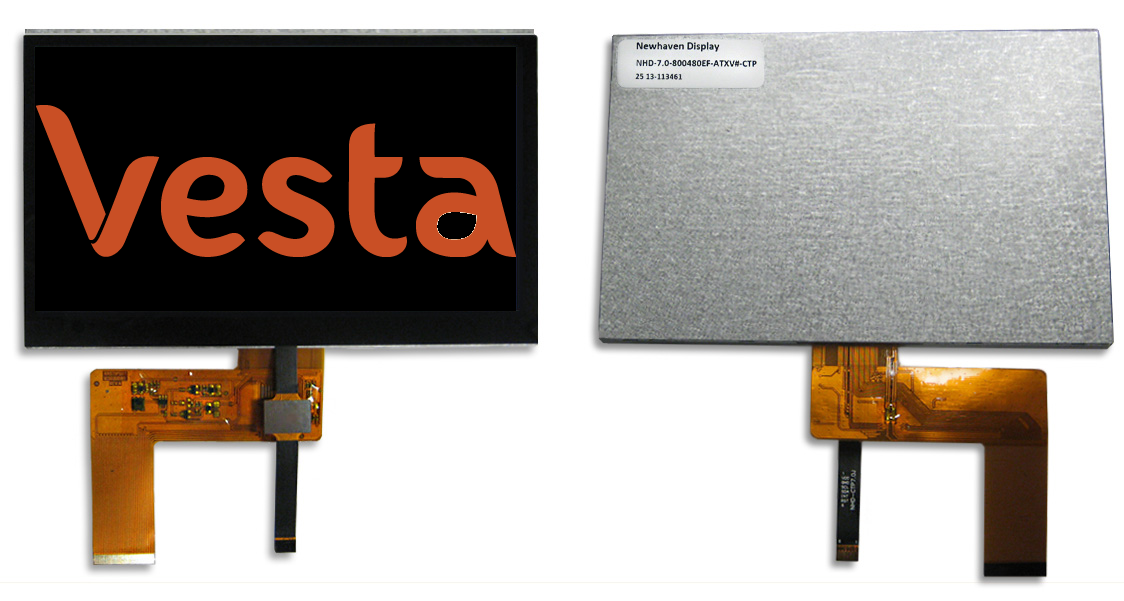
\includegraphics[width=0.5\textwidth,keepaspectratio]{chap/hardFig/newhaven_screen_image}
     \caption{Screen package.}
     \label{fig:screen package}
 \end{figure}

 Individual components are discribed in the following sub chapters.

\subsubsection{Screen}
The screen is the NHD-7.0-800480EF-ATXV\#-CTP from Newhaven Display. The specifications of the screens are listed bellow.
\begin{itemize}
  \item {7" Diagonal}
  \item{Resolution: 800xRGBx480}
  \item{24 bit digital RGB interface}
  \item{White led backlight}
  \item{55-65$^{\circ}$ Top-bottom viewing angle }
  \item{70 $^{\circ}$ left-rigth viewing angle}
  \item{}
\end{itemize}


\subsubsection{Touchscreen}

\begin{itemize}
  \item {Capacitive touch panel with built-in Focaltech ft5x06 controller}
  \item {i2c interface}
  \item {linux kernel compatible}
\end{itemize}
The touchpanel is very smooth and reactive. The
\subsubsection{Backlight}
The backlight is a quite bright white led array consisting of 5x3 LEDs. the configuration can be seen in fig.\ref{fig:backlight_led}

\begin{figure}[!htb]
    \centering
    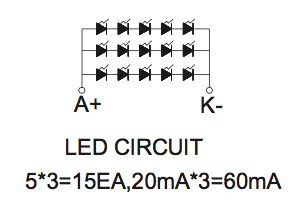
\includegraphics[width=0.5\textwidth,keepaspectratio]{chap/hardFig/backlight_led_circuit}
    \caption{Backlight LED array configuration.}
    \label{fig:backlight_led}
\end{figure}

This LED array requires 60 mA at 16 V to operate. This power is taken directly from the 3.3v of the BBB and boosted to the required voltage by FAN5333A LED driver from Fairchild semiconductors.
This IC is a general purpose LED driver which can be controller with a PWM imput.
Our implementation of the FAN5333A is pictured in fig.\ref{fig:backlight driver schematics}.

\begin{figure}[!htb]
    \centering
    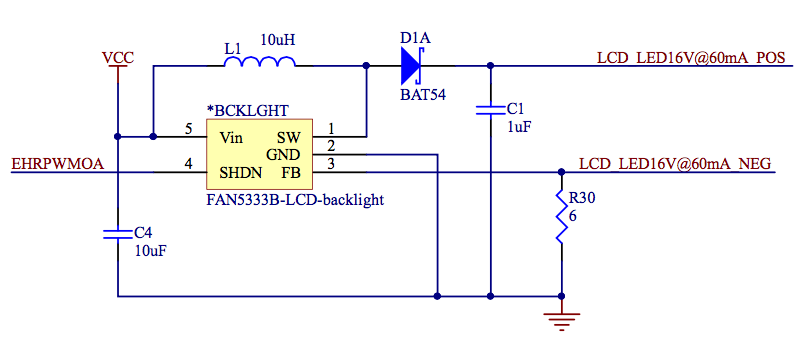
\includegraphics[width=0.7\textwidth,keepaspectratio]{chap/hardFig/backlight_led_driver_sch}
    \caption{FAN5333A Backlight LED driver implementation.}
    \label{fig:backlight driver schematics}
\end{figure}

From the data sheet the resistance R30 sets the current. The net EHRPWMMOA is connected to a pwm pin on the BBB.
\subsection{Wireless Communication}
Our device has to connect to the internet over a WLAN to download new messages from the website. We chose to use the WL1835 chip from Texas instruments. This IC integrates WlAN, bluetooth and low energy bluetooth.
\subsubsection{Wlan}
The chip supports the IEEE standards 802.11a/b/g/n. This means it can provide up to 100 MPs with UDP and up to 80 MPs with TCP.
It uses a 4 bit SDIO interface to communicate with the BBB.
\subsubsection{Bluetooth}
The Wl1835 provides 4.1 bluetooth and low energy bluetooth capabilities. Uart host controlled interface is used here.
\subsubsection{Power management}
The WL1835 is quite power hungry and requires both 3.3V and 1.8V to operate. Therefore it has its own linear regulators.
\subsection{Front LED}
The LED is there to inform the user of a new message. Therefor it could be quite low power. Seeedstudio only had an RGB LED which we ordered although for the final led we will use is a warm white single color LED.

We want it to flash in a heartbeat patern. This is achieved by using a PWM pin of the BBB
\subsection{Power management}
\subsection{Batteries and charger}
\subsection{PCB}
\subsection{Cost estimates}

\section{Software}
%\subsection{Description}
The software of this project contains 3 parts:
\begin{itemize}
\item{The operating system configuration and modification to be fully compatible with the hardware used.}
\item{The website that is used by the young users to send pictures and messages to the old users.}
\item{The Vesta tab software that is used on the tablet to display the differents messages and pictures received by the old users.}
\end{itemize}

The concept of this software is easy to understand. Every tablet has a unique id like a phone number. The young user knows this id and can send messages and pictures to the wanted tablet through the website. The tablet just needs to be configured to connect to the wifi and get messages sent by the young user. The old people has almost nothing to do, the pictures are displayed automatically. He can naviguate in the old messages by swiping the pictures on the tablet.

It is similar to a digital photo frame but the pictures are not put on the tablet by the tablet owner but by the young user.

The figure \ref{fig:web connections} shows the web interactions between the website and the Vesta software on the tablet.

\begin{figure}[!htb]
    \centering
    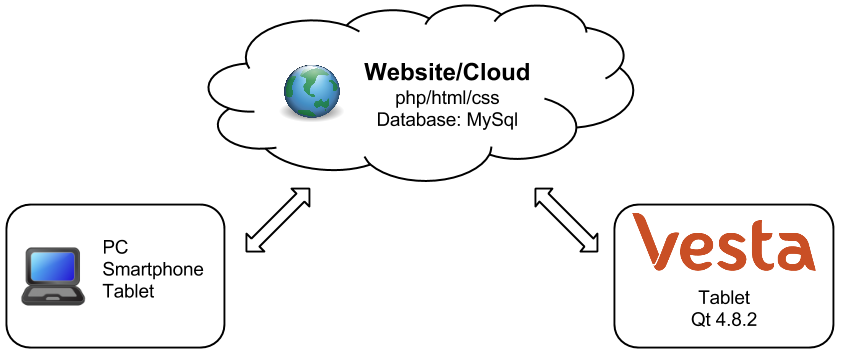
\includegraphics[width=0.9\textwidth,keepaspectratio]{chap/softFig/web_connections.png}
    \caption{Web connections}
    \label{fig:web connections}
\end{figure}

\clearpage

The figure \ref{fig:user flow} shows the interactions between the website and the Vesta software on the tablet. All the files are stored on the website on the mySQL database. When the pictures are sent, the vesta tablet receives a message and can open/display it. The vesta software on the tablet works on a linux OS that manages the hardware.

\begin{figure}[!htb]
    \centering
    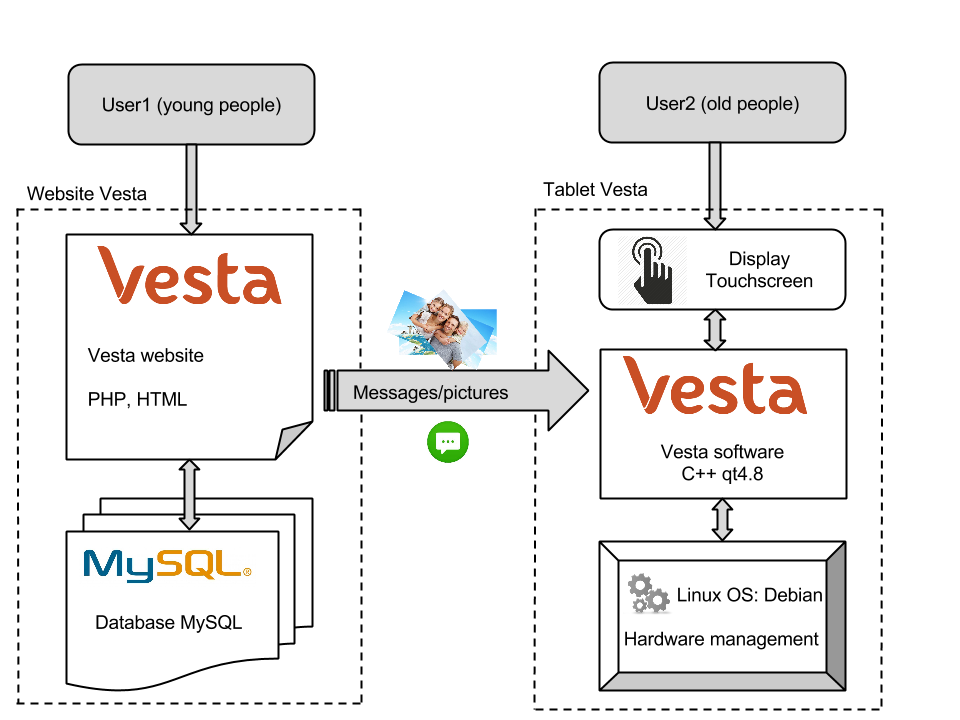
\includegraphics[width=0.9\textwidth,keepaspectratio]{chap/softFig/block_diagram_vesta2.png}
    \caption{Basic user flow.}
    \label{fig:user flow}
\end{figure}

\clearpage

\subsection{Operating system}
The OS used for this project is a debian. Debian is a linux distribution and was given by the conceptors of the beaglebone black.

The original OS is available on the beaglebone black developer website: http://beagleboard.org/latest-images

The figure \ref{fig:OS} shows how the are the interactions between the OS and the hardware or the software.
 
\begin{figure}[!htb]
    \centering
    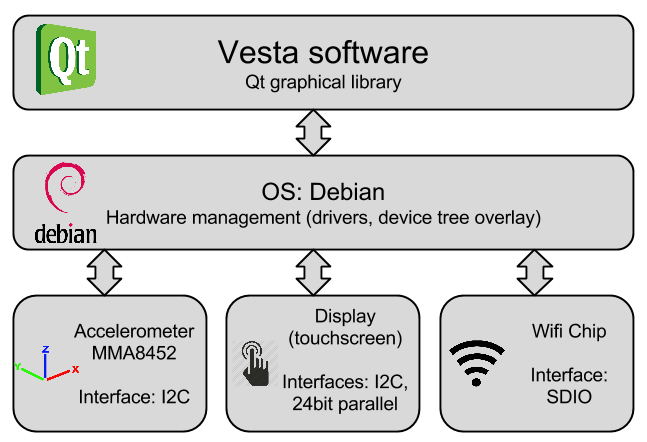
\includegraphics[width=0.7\textwidth,keepaspectratio]{chap/softFig/first_diagram2}
    \caption{Interactions between the operating system and the hardware/software.}
    \label{fig:OS}
\end{figure}

The original OS contains:
\begin{itemize}
\item{kernel 3.8: The linux kernel (an old one)}
\item{X11: The graphical server}
\item{lxdm: The user session management}
\item{lxde: A desktop (light)}
\end{itemize}

The OS manages the communications with the different hardware. The accelerometer is controled by I2C (to read datas and write configurations). The screen uses different interfaces, I2C for the touch panel and 24bit parallel for the display. The WIFI chip is connected with SDIO and it replaces the emmc memory.

Every protocol and every pins input or output have to be declared in a file called device tree source. In the 3.14 kernel, this file is compiled and become a device tree blob. The compiled version of the file is executed at the OS startup. It initiates the load of the drivers and configures the pins as input, output, pwm or interrupt. Some pins can be configured as i2c, spi, SDIO or some other protocols.


Packets installed on the original debian OS:
\begin{itemize}
\item{libqt4-core: Defaults tools for Qt software execution}
\item{libqt4-gui: Needed to display GUI software developped with Qt}
\item{dtc: Device tree compiler used to create pin configuration at the OS startup}
\item{wicd: Network manager for WIFI connections}
\item{evtest: Tool for interruption event, used especially to debug the touchscreen}
\end{itemize}


\subsubsection{Drivers}
A lot of work on this linux distribution was made to be fully compatible with the chosen hardware.
The touch screen driver edt-ft5x06 had problems with the original 3.8 kernel of the distribution used. The driver was not loading correctly from the device tree overlay. An upgrade to the 3.14 kernel resolved the problem.
Then the scale of the touchscreen was not correct. 
When a touch event occured on the right-down corner, the mouse pointer moved to the center of the screen. Some configuration scripts had to be modified for the X11 graphical display server.

The edt-ft5x06 uses an interrupt line and I2C to get the touch events and the positions of the clicks.

Another driver is used for the WIFI connection with the wl1835mod. This driver uses the protocol SDIO. It also has to be declared and initialized at the OS startup in the device tree blob. As the beaglebone's processor has only one SDIO protocol possible and it is used by the emmc memory, the emmc is replaced by the WIFI chip and the emmc is unusable.

\subsubsection{Display}
The touch screen works with a 24 bits parallel interface so the X11 configuration file had to be modified to work correctly. The LCD output was initialy configured in 16 bits parallel interface.
The hardware management in linux is called a device tree blob. It’s a script that is compiled and is loaded at the OS startup. In this file, the driver for the touch panel was declared and the interrupt pins was defined. The resolution and frequency of the display is also configured in this script. The wifi chip also needs to load drivers at startup and tell the OS to connect to internet via this chip and with the SDIO protocol.
The file is located in /boot/dtbs/3.14xx/ and is called vesta.dtb (compiled) and the source is called vesta.dts. The file uEnv.txt located in /boot/ also needs to define which device tree blob(dtb) the OS has to load at startup.

\clearpage

\subsection{Website}

The website is used by the young users to send messages and pictures to the old user’s tablet.
The website contains a MySQL database, a php/html page that let the young user send a message and a php script used to parse the database to XML to be readable by the tablet.

The figure \ref{fig:web archi} shows the architecture of the interactions between the webpage, the database and the connections by the tablet through a script.

\begin{figure}[!htb]
    \centering
    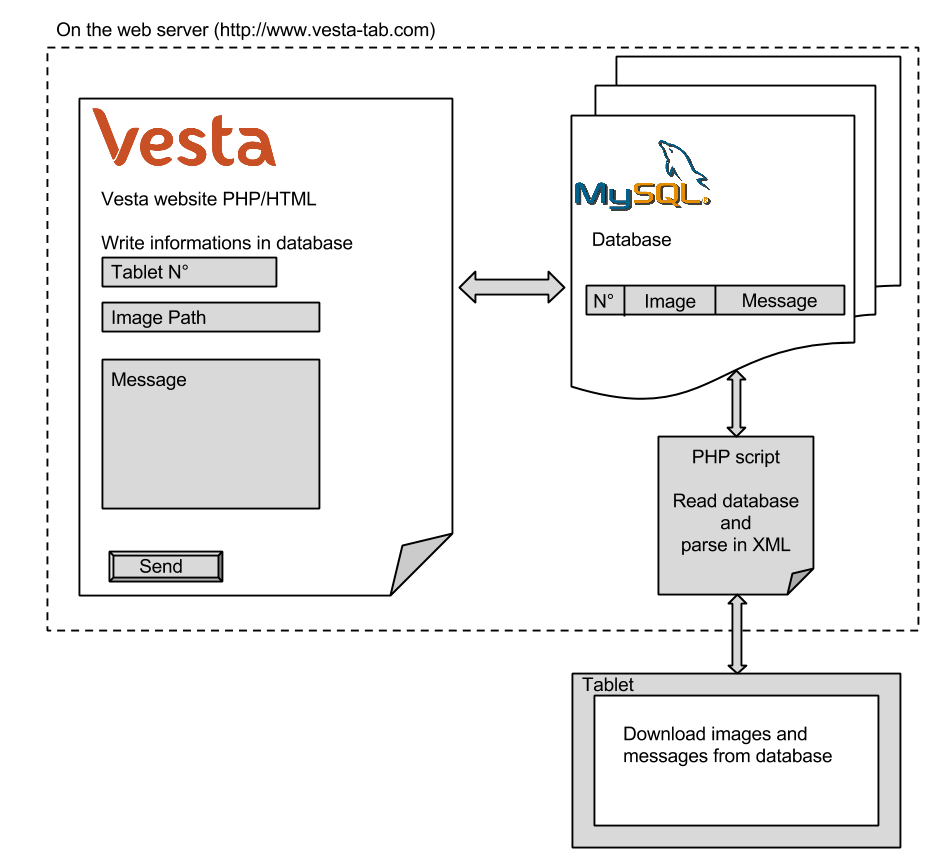
\includegraphics[width=0.9\textwidth,keepaspectratio]{chap/softFig/vesta_website2}
    \caption{Vesta website architecture.}
    \label{fig:web archi}
\end{figure}

\clearpage

\subsubsection{Webpage}
The webpage let the young user send a message to a wanted tablet. Every tablet has an id like a phone number known by the tablet owner. It is possible to select a picture on the user's computer and write a text message. When the "send" button is clicked, the picture and text message is saved in the MySQL database.

The php script called when the send button is clicked downloads the picture contained in the file input, verify if the file downloaded is a picture and if the size is not too big. If everything went well the picture and the other datas are saved in the MySQL database else some error messages are displayed. The date is automatically written at the current time.

\clearpage

\subsubsection{Database and XML parsing}
The MySQL database is where all the messages and pictures are stored. The webpage connects and save the datas into the database when the user send a message.

An example of entries on the vesta table on the MySQL database are shown in the table\ref{tab:database}.

\begin{table}
\begin{tabular}{|c|c|c|c|c|c|c|}
  \hline
  id & type & name & sender & text & img & date \\
  \hline
  7 & image/jpeg & family.jpg & Jean & Hello! A message for you & BLOB - 300KB & 14.05.2015\\
  8 & image/jpeg & cat.jpg & Marie & Look at my cat :) & BLOB - 350KB & 27.05.2015\\
  \hline
\end{tabular}
\caption {Example of entries in the vesta table on the MySQL database}\label{tab:database}
\end{table}

When the tablet update the datas, it connects to a script contained on the server. This script connects to the database and parse the informations needed by the tablet in XML.The tablet then unparse the datas, downloads the pictures, and displays them.

XML is a markup language that facilitates the transfer of datas and the readability of them. It is mainly used in the RSS flux.


An example of XML code is shown below:

\lstset{
style=customxml,
 basicstyle=\ttfamily,
 columns=fullflexible,
 showstringspaces=false,
 commentstyle=\color{green}\upshape
}


\begin{lstlisting}
<?xml version="1.0"?>
<vesta>
  <item>
    <title>family.jpg</title>
    <sender>Jean</sender>
    <date>2015-04-18 17:08:45</date>    
    <image>http://www.vesta-tab.com/jo/getImage.php?id=7</image>
    <message>Hello! A message for you</message>
  </item>
  <item>
    <title>cat.jpg</title>
    <sender>Marie</sender>
    <date>2015-04-23 14:34:12</date>
    <image>http://www.vesta-tab.com/jo/getImage.php?id=8</image>
    <message>Look at my cat</message>
  </item>
</vesta>
\end{lstlisting}

This XML file defines 2 messages: family.jpg and cat.jpg. The senders are Jean and Marie at respectively 17:08:45 the 18th april 2015 and 14:34:12 the 23th april 2015. The images are available at the URL defined between the image markups. The message is between the message markups.

\clearpage

\subsection{Vesta software on the tablet}
The Vesta software is used by the old users to receive and display the messages and pictures sent by the young users. It is located on the tablet and working with debian. The software is made in C++ with Qt4.8/Qt quick 1.0.

\subsubsection{Qt library}
Qt is a free library used mainly to design softwares with graphical user interfaces (GUI). It is cross platform so with the same code it is possible to compile for linux,windows and mac.
The library contains also a lot of utils to facilitate the development of emmbedded interfaces and manages the touchscreen events like the swipes, clicks and more. A lot of documentation is available and a lot of users develop with it.

There are differents GUI library like Gtk+, CEGUI etc... The choice of Qt was done especially because it is cross platform but also because it's compatible with emmbedded systems. Qt can be used also with android and IOS and is really made for apps with touchscreen. Qt quick is very powerful for emmbedded applications. The last version of Qt was downloaded over 1 million times and is ranked number 1 of all cross-platform tools.

Qt creator is the official development environnment for Qt. It is used to develop and cross-compile the software for the beaglebone black. A visual GUI editor is available and simplify grandly the development of the software GUI.

\clearpage

\subsubsection{Overall operations}
At the startup, the vesta tab init and check the wifi connection. The touchscreen creates an event when someone touch it and changes the image displayed. It lets the user naviguate between the different messages. Every minute the soft check if a new message is received.

The software is quite simple and not a lot of functionnalities are implemented. The goal was to have a really easy to use software for old people.

The figure \ref{fig:soft archi} shows how the software works.

\begin{figure}[!htb]
    \centering
    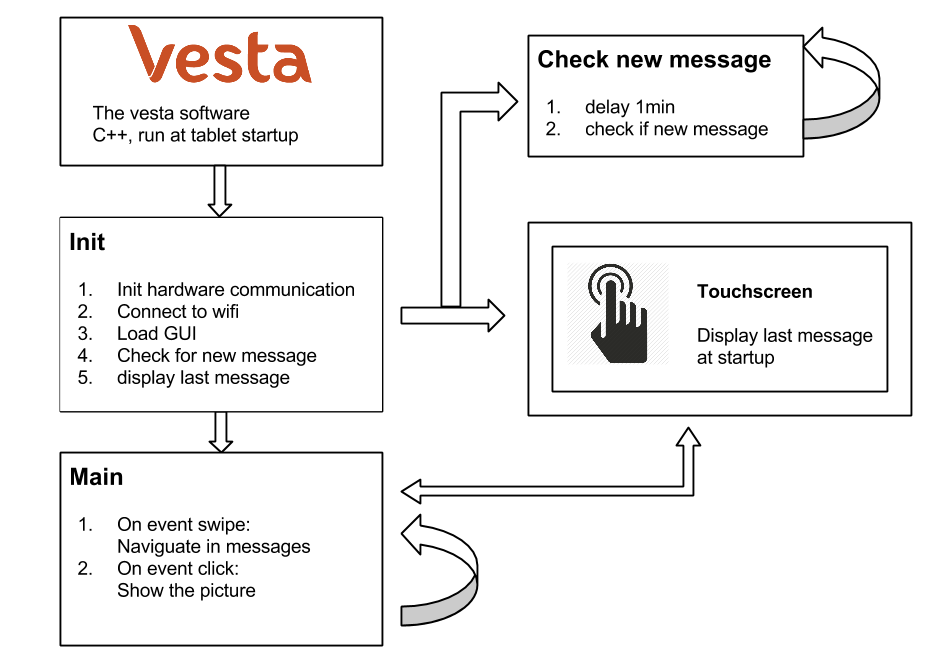
\includegraphics[width=0.9\textwidth,keepaspectratio]{chap/softFig/vesta_software_diagram2}
    \caption{Vesta software architecture.}
    \label{fig:soft archi}
\end{figure}

\clearpage

\subsubsection{Graphical interface}
The graphical interface is composed of an horizontal listview and some buttons. The listview allows swipes event to naviguate between the different pictures and messages.

A task bar is always visible on the top of the GUI. The list view displays the actual picture, the date when the messages was sent and the text message.

The figure \ref{fig:gui diagram} shows how the GUI is constructed.

\begin{figure}[!htb]
    \centering
    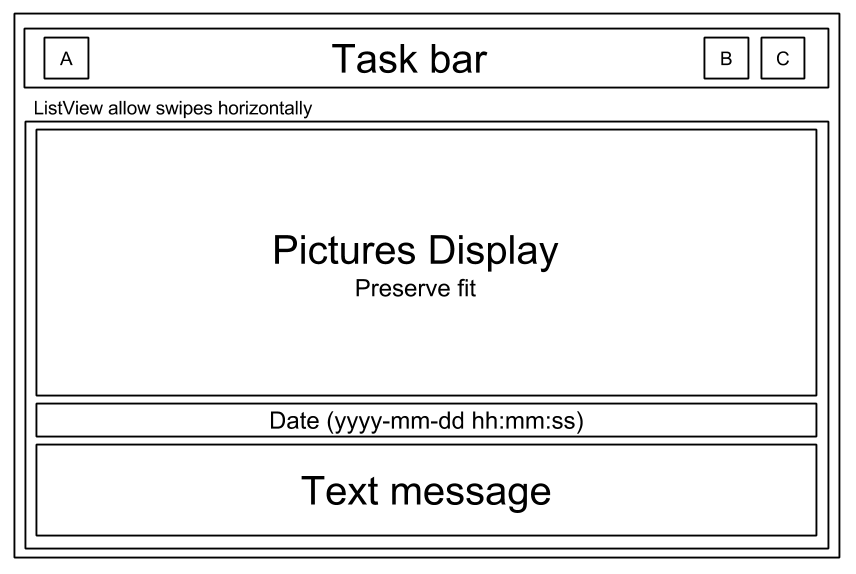
\includegraphics[width=0.7\textwidth,keepaspectratio]{chap/softFig/GUI_diagram}
    \caption{Graphical interface diagram, A:Refresh button, B:WIFI RSSI indicator, C:Battery state indicator}
    \label{fig:gui diagram}
\end{figure}

The buttons let the user configure the wifi or display the new messages.

\begin{itemize}
\item{The button A refresh the messages and display the last one.}
\item{The button B goes to the WIFI configuration and indicates the RSSI of the WIFI.}
\item{The indicator C show the battery level}
\end{itemize}

The figure \ref{fig:graphical interface} shows the actual GUI.

\begin{figure}[!htb]
    \centering
    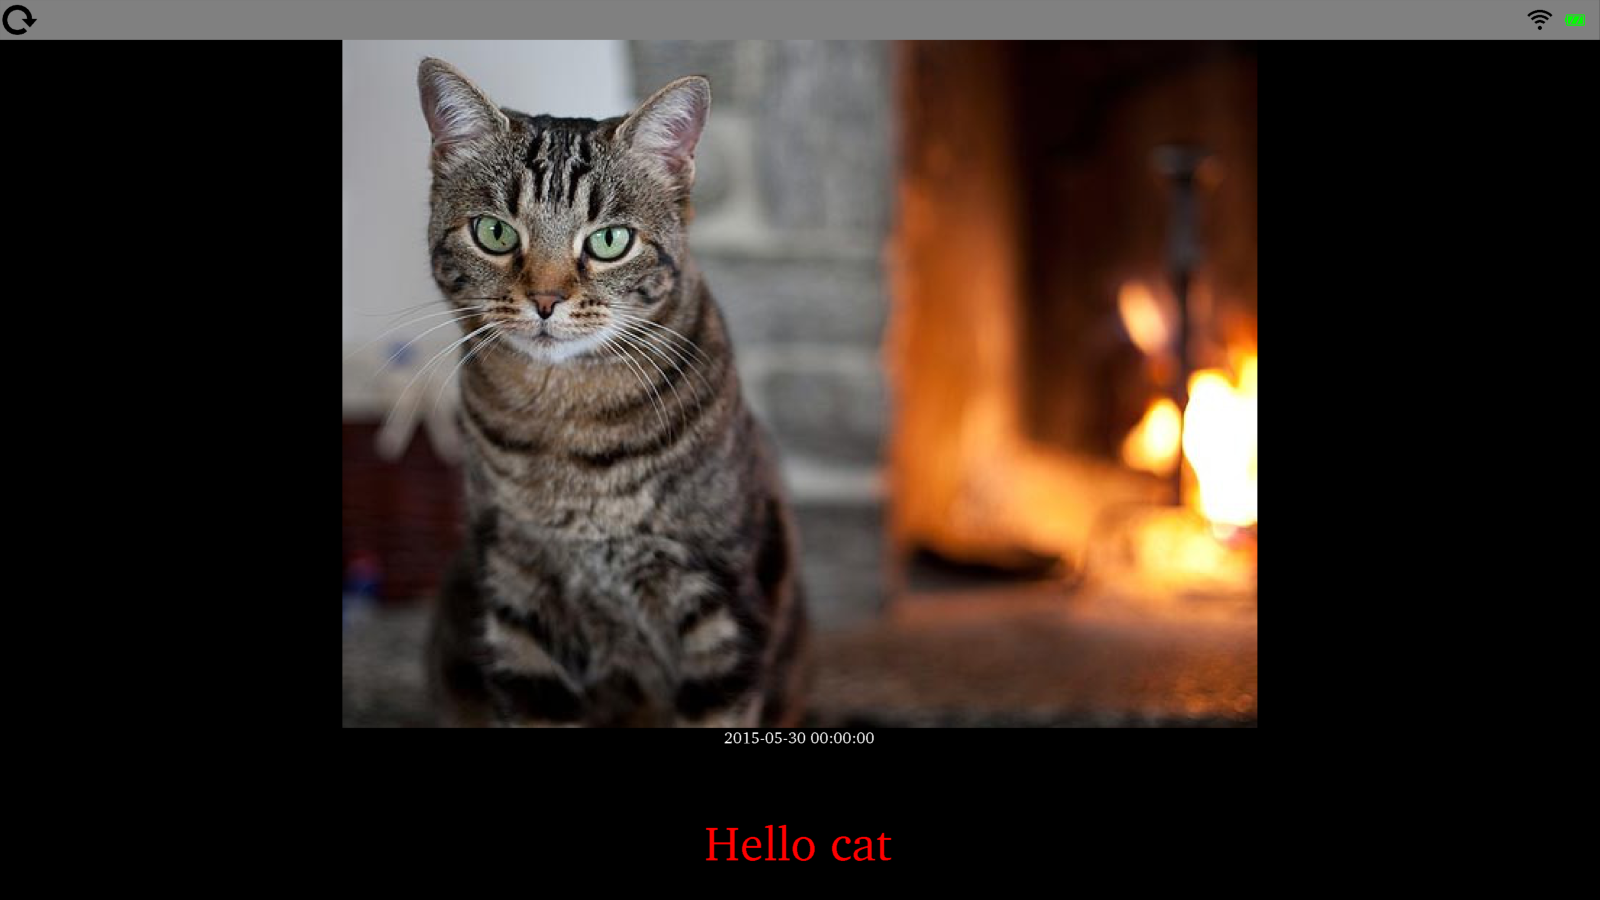
\includegraphics[width=0.7\textwidth,keepaspectratio]{chap/softFig/vesta_printscreen}
    \caption{Vesta software graphical interface}
    \label{fig:graphical interface}
\end{figure}



\section{Next steps}
\label{chap: next steps}

In the beginning of july, a first prototype will be made in Shenzen (China) with an industrial partner (Seeedstudio). A final presentation of the project is going to take place in october with the prototypes.

A lot of fonctionnalities could be easily implemented after this prototyping step. An activity monitoring or an emergency call system for example. Another fonctionnality can be a videoconference system with a camera like Skype does. This device has a lot of unused connections that could be used to connect other sensors for medical assistance for example. It could become a connected electrocardiogram monitor. The advantage is that the hardware is powerful enough to do almost everything a computer can do in term of connectivity. Everything that can be done with a tablet can be done with this device and more.

The device contains bluetooth integrated in the wl1835 chip and is not currently used. Bluetooth could be used to have more interactions with other devices or to configure the tablet. For example the configuration and selection of the WIFI network can be done via an app on a smartphone with bluetooth. Or an activity tracker bracelet could upload the data to the tablet. The tablet would be used to display the activity in some plots. The family would have a remote monitoring facility.

The software can be changed relatively easily to do a completely different task. Qt is a well known library that let the programmer creates interfaces very fast. This device may become a developpement board.

Currently the only way to send messages or pictures is trough the website. A next step could be to develop an app on IOS and android to send pictures directly from a smartphone or a tablet.

\section{Problems encountered}

The main problems encountered were about the OS configuration and compatibility with the hardware components. The driver for the I2C capacitive touch panel chip wasn't working with the kernel 3.8. The driver was loading at the OS startup but no input was available to read it. This problem was resolved by upgrading the kernel to the 3.14 version. The scale of the touchscreen was also not working. The events were readable but they were wrong, the clicks were not synchronized with the screen size. Some calibration configurations of the X11 config file resolved the problem.

Having no knowledge of PCB design prior to this project, the learning curve was steep. Information was sometimes sparse on specific subjects such as for the antenna footprints.

Getting information on some parts especially from chinese providers was sometimes impossible. For these reasons some of the parts were very expensive.

\section{Conclusion}

The software is not finished yet but the hardware and design is already well implemented. The priority was placed on the hardware and the design. These two parts must be finished before going to China but the software can be finished afterwards.


%----------------------------------------
% Annexest
%----------------------------------------

\begin{comment}
\appendix
	\setcounter{page}{1}
	\pagenumbering{Roman}
		%---- Liste des tableaux et des figures ----%
%\listoftables
%\listoffigures
	%\clearpage

	%---- Glossaire ----%
	%Mise en forme de la liste du glossaire
	\renewenvironment{glosslist}
	{\begin{liste_glossaire}}
	{\end{liste_glossaire}}
	%Met dans le glossaire tous les éléments non directement cités dans le texte
	\gloss[nocite]{*}
	%Efface le titre pour chaque nouvelle lettre
	\renewcommand{\glossheading}[1]{}
	\printgloss{glossaire}
	%\clearpage

	%---- Bibliographie ----%
	% Citer tous les ouvrages/références
	\nocite{*}
	% Type de bibliographie : non-triée
	\bibliographystyle{unsrt-fr}
	\bibliography{biblio}
	\addcontentsline{toc}{section}{Références}
	%\clearpage

	%---- Index ----%
	\printindex
\end{comment}

\end{document}
